%% This is an example first chapter.  You should put chapter/appendix that you
%% write into a separate file, and add a line \include{yourfilename} to
%% main.tex, where `yourfilename.tex' is the name of the chapter/appendix file.
%% You can process specific files by typing their names in at the
%% \files=
%% prompt when you run the file main.tex through LaTeX.
\chapter{Literature}

In this chapter there will be an extensive explanation to the technologies used
throughout the document.

\section{Internet of Things}

What is the \textbf{\textit{Internet of Things}}?\\
\textit{Internet of Things}, better known as IoT, is the world of interconnected devices
connected to the real world and to the Internet. These devices has a very
broad definition, from the smart sensors in a power plant to the smart fridge in
a house. What connects these devices is their ability to be connected with the world,
sharing, with the needed restrictions, their work. This opened the door to a new
revolution in the IT sector, prompting new opportunities for developers, entrepreneurs
and end users. Some of the most relevant endings of these technologies are \textit{Smart Houses},
\textit{Smart Cities}, Cars etc. %[TODO] continue a little bit here

\subsection{Ecosystems}

What is an Ecosystem? An ecosystems is by definition \textit{a system, or a group of interconnected elements,
formed by the interaction of a community of organisms with their environment.},
in our case a set of smart devices connected between them. The IoT world is evolving
from distinct single entities to more evolved clusters of devices which can communicate
more easily between each other.These are usually are made by companies using specific protocols or standards
to simplify the connection between their products, but at the same time closing it to the others.
%[TODO] connect the two paragraphs
The list of products related to the \textit{Internet of Things} is too broad for
being even listed, due to the highly expanding sector related to smart devices.
However we will consider the most common ecosystems which can be easily found in a common
home, meaning services for: Smart Lights, Cameras, Thermostats etc. Luckily
most of them are being bought and integrated in bigger environments run by
famous companies such as \textit{Google} or \textit{Apple}.
The reason for which we try to restrict the integration with these ecosystems is
mainly practical, because they're the most common and they do offer simulators
for testing, and because they suits perfectly our scenario.

%[TODO] describe the various ecosystems, what is an ecosystem etc
\subsubsection{Google - Nest}

\textbf{Nest} is a home automation producer of smart devices
which ranges from their famous Smart Thermostat to the locking system, from the
washing machine to the light system, from the \textit{Dropcamera} to the Hi-Fi Sound system,and
these are just some examples. The number of components supported by this company
is wide, which makes it a good choice to support in our scenario, also because of
the high cost of these devices. The main added value given by these accessories is related
to two main points: saving money with a smart consumption of electricity using data analytics and being
able to remotely control the house with an easy to use application.
Besides the commercial value of \textit{Nest}, the platform offers many tools for developers
to interact with their platform with their Cloud service. Third party developers
are encouraged, with some limitations, to interact with their Cloud service which
offers some \textit{RESTful} APIs to gather access to the remote devices.

\subsubsection{Apple - HomeKit}
\subsubsection{Samsung - SmartThings}


\section{Calvin}



\section{The Microservice Architectural Style}

\subsubsection{SOA vs Microservices}
In short, the \textit{microservice architectural style} is an approach to developing a single
application as a suite of small services, each running in its own process and communicating with
lightweight mechanisms, often an HTTP resource API. These services are built around business capabilities
and independently deployable by fully automated deployment machinery. There is
a bare minimum of centralized management of these services,
which may be written in different programming languages and use different data storage technologies.[7]\\
There is a close link between the \textit{microservice architecture} and the \textit{service oriented architecture},
thus due to their nature the community classified microservices as a subclass of the service oriented architecture.
\textit{Don Box} of Microsoft described the Service-Oriented paradigm with the following four principles [8]

\begin{enumerate}
  \item Boundaries are explicit
  \item Services are autonomous
  \item Services share schema and contracts, not class
  \item Service compatibility is based on policy
\end{enumerate}

Microservices fullfills the first two requirements, with a very strong focus on the second principle.
However the functionalities are very frequently exposed using a \textit{RESTful} interface, which
doesn't expose any contract nor schema. Furthermore microservices holds another subtle difference related to their
scope, where a microservice serves as a service inside its application meanwhile typical SOA services
serves a broader scope and \textit{can be} part of the same application.
The difference between the two concepts is very subtle, and it wouldn't be impossible for them
to be the same in certain situations. \textit{Bob Ruhbart} from Oracle described shortly the difference:
\textit{Microservices are the kind of SOA we have been talking about for the last decade. Microservices must be independently deployable,
whereas SOA services are often implemented in deployment monoliths.
Classic SOA is more platform driven, so microservices offer more choices
in all dimensions}.[10]

\begin{figure}[h]
\caption{Graphic illustration of microservices and SOA}
\centering
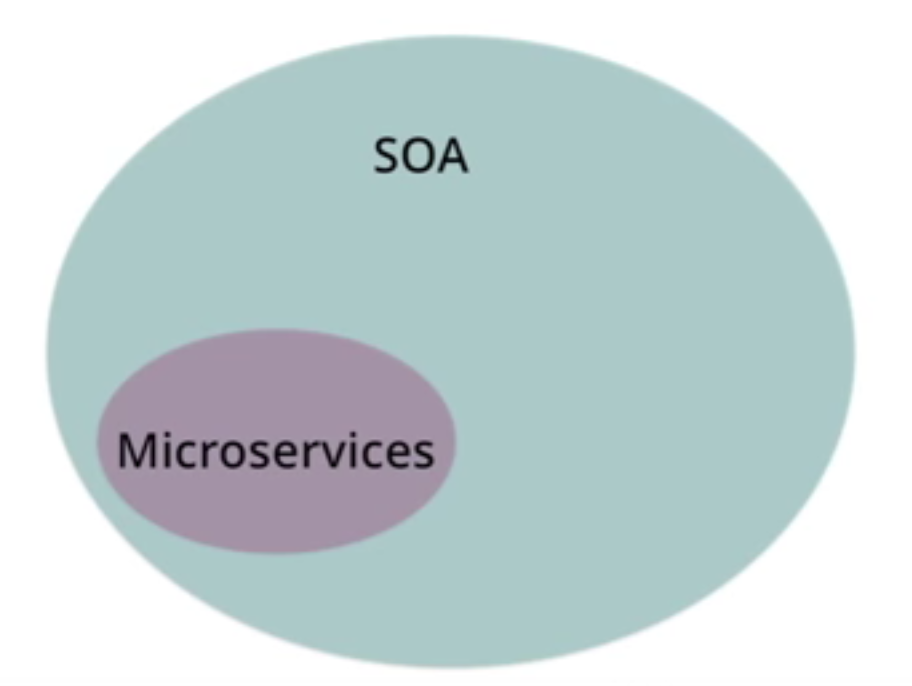
\includegraphics[scale=1]{soavsmicro.png}
\end{figure}

\subsection{Internal integration}
%[TODO] IMPROVE!!!!
Typically when a new component has to be added to an existing
project the approach consists in the development of a library which
has the logic to deal with the new module to be supported. Subsequently the component
will
become part of the project itself, with its needs to be updated when needed.
However when the number of components to integrate increases will affect the size
of the project and its performances, introducing scalability problems.
In our case the module to be integrated will be the ecosystem taken in consideration,
having a set of libraries which are capable of interacting with the remote APIs or
with the direct wired connections.

\subsection{Integration as a Service}
Considering the \textit{Microservice} architectural pattern we can decompose
the above situation creating dedicated services capable of handling the
required business logic to interact with an external system. This approach
is also called \textbf{Componentization via Services}[7], where a component is defined
as a \textit{unit of software that is independently replaceable and upgradeable.}
It is important to distinguish between \textit{libraries} and \textit{services}:
the latter uses out-of-service components to communicate, mainly HTTP requests or
remote procedure calls when libraries uses instead mechanisms like in-memory calls.
The main advantage to build components as services instead of libraries is the
possibility to deploy them individually without the need to redeploy the whole system.
If a library is modified or removed the whole system will need to be redeployed,
which in most of the cases it is converted in a loss of money and time. That's not
the case if the system is composed by many independent systems, where only the changed
service will need a new deployment. However this is not always true, there will be some
circumstances where it will be necessary anyway to deploy again the whole system, but the
aim of this approach is to reduce the number of these necessities.

\subsection{Main benefits}

\begin{description}
  \item[Heterogeneity between technologies] Structuring the system as a set
  of services frees us from the limitations of a singular technology allowing
  us to adopt different frameworks for different tasks. This benefits on the
  possible optimization that can be achieved using the right technology for the
  right task. Furthermore this removes completely the problem of creating adapters
  for different technologies to integrate in the system if they do not exist.
  \item[Evolutionary Design] is a typical feature of microservice
  architecture where components can be easily upgraded or redeployed.
  Decomposing the system as a set of many independent components allows us
  to upgrade a service without affecting the core components and redeploying
  the whole project. This allows us to upgrade, use different technologies, modify
  or remove our component without any consequence on the rest of the system.

\end{description}
